\chapter{Absolute extensors and absolute neighborhood extensors}

In this section we will study \aexs\ and \anes, because they are strongly connected to \ars\ and \anrs. The connection is stated in \ref{theorem:ane_to_anr} and \ref{theorem:anr_to_ane}. 

\begin{definition}
	A topological space $\tspace[Y][O]$ is called \textit{\aex} for a full subcategory $\cat$ of $\Top$, if and only if for every closed set $A$ of an object $\tspace$ of $\cat$ and every $f \in \Hom_\Top\pbraces{\reltspace, \tspace[Y][O]}$ there exists an extension $\overline{f} \in \Hom_\Top\pbraces{\tspace, \tspace[Y][O]}$ of $f$.  
\end{definition}

\begin{definition}
	A topological space $\tspace[Y][O]$ is called \textit{\ane} for a full subcategory $\cat$ of $\Top$, if and only if for every closed subset $A$ of an object $\tspace$ of $\cat$ and every $f \in \Hom_\Top\pbraces{\reltspace, \tspace[Y][O]}$ there exists a neighborhood $U$ of $A$ in $\tspace$ and an extension $\overline{f} \in \Hom_\Top\pbraces{\reltspace[U], \tspace[Y][O]}$ of $f$.
\end{definition}

\begin{proposition}
	Every \aex\ for a full subcategory $\cat$ of $\Top$ ia an \ane\ for $\cat$. 
\end{proposition}
\begin{proof}
	Let $\tspace[Y][O]$ be any \aex\ for $\cat$ and consider any closed set $A$ of an object $\tspace$ of $\cat$ and any $f \in \Hom_\Top\pbraces{\reltspace, \tspace[Y][O]}$. Since $\tspace[Y][O]$ is an \aex\ for $\cat$, there exists an extension $\overline{f} \in \Hom_\Top\pbraces{\tspace, \tspace[Y][O]}$ of $f$. This concludes the proof, because $X$ is a neighborhood of $A$ in $\tspace$. 
\end{proof}

\begin{proposition}
	Every \aex\ (respectively \ane) for a full subcategory $\cat$ of $\Top$ is also an \aex\ (respectively \ane) for every full subcategory $\mathcal{C}$ of $\cat$. 
\end{proposition}
\begin{proof}
	We will proof the statement only for \anes, because the proof for \aexs\ is similar. Let $\tspace[Y][O]$ be an \ane\ for $\cat$. Let $A$ be a closed set of any object $\tspace$ of $\mathcal{C}$ and $f \in \Hom_\Top\pbraces{\reltspace, \tspace[Y][O]}$. Since $\tspace[Y][O]$ is an \ane\ for $\cat$, there exists a neighborhood $U$ of $A$ in $\tspace[Y][O]$ and an extension $\overline{f} \in \Hom_\Top\pbraces{\reltspace[U], \tspace[Y][O]}$ of $f$. Thus, $\tspace[Y][O]$ is an \ane\ for $\mathcal{C}$ and the proof is complete.
\end{proof}

\begin{proposition}
	If a subcategory $\cat$ of $\Top$ contains an object which does not fulfill \ref{axiom:t4}, then every \ane\ $\tspace$ for $\cat$ which is Hausdorff¸ consists  of a single point. \colorbox{red}{or $X = \emptyset$ and $\mathcal{T} = \Bbraces{\emptyset}$ ?}
\end{proposition}
\begin{proof}
	Assume there exists a Hausdorff space $\tspace[Y][O]$ which is an \ane\ for $\cat$ that contains two distinct points $y_1, y_2 \in Y$. There exists an object $\tspace$ of $\cat$ which is not normal, hence there are two disjoint closed sets $B$ and $C$ of $\tspace$ which can not be separated by neighborhoods. The set $A := B \cup C$ is closed in $\tspace$, because it is the union of two closed sets. We define a function $f: A \to Y$ by
	\begin{align*}
		f(x) := 
		\begin{cases}
			y_1 &, \text{if } x \in B \\
			y_2 &, \text{if } x \in C
		\end{cases}
	\end{align*} 
	\colorbox{red}{Show that $f \in \Hom_\Top\pbraces{\reltspace, \tspace[Y][O]}$.} Since $\tspace[Y][O]$ is an \ane\ for the class $\cat$, there exists a neighborhood $U$ of $A$ in $\tspace$ and an extension $\overline{f} \in \Hom_\Top\pbraces{\reltspace[U], \tspace[Y][O]}$ of $f$. Since $\tspace[Y][O]$ is Hausdorff, we find a neighborhood $V$ of $y_1$ and a neighborhood $W$ of $y_2$ such that $V \cap W = \emptyset$. Therefore, $g^{-1}\bbraces{V}$ is a neighborhood of $B$ in $\reltspace[U]$, the set $g^{-1}\bbraces{W}$ is a neighborhood of $C$ in $\reltspace[U]$ and $g^{-1}\bbraces{V} \cap g^{-1}\bbraces{W} = \emptyset$. Thus we separated $B$ and $C$ by neighborhoods, which clearly is a contradiction that concludes the proof. 
\end{proof}

The following theorem provides us with a great number of examples of \aexs\ and hence also \anes. 

\begin{theorem}[Dugundji extension theorem]
	Every convex subset of a locally convex topological vector space is an \aex\ for $\Met$.
\end{theorem}

\begin{proof}
	Let $C$ be a convex subset of an object $\tvspace{\K}$ of $\LCTVS{\K}$ and let $\tspace$ be an object of $\Met$. Consider any arbitrary closed set $A$ in $\tspace$ and a continuous function $f \in \Hom_\Met\pbraces{\reltspace, \reltspace[C][O]}$. The set $\cover := \Bbraces{\ball[x][2^{-1} \dist\pbraces{x, A}] \mid x \in X \setminus A}$ is an open cover of $\reltspace[X\setminus A][T]$. 
	
	The metrizable space $\reltspace[X \setminus A][T]$ is paracompact by \ref{theorem:stone}, hence there exists a locally finite refinement $\cover[V]$ of $\cover$ which covers $X \setminus A$. By \ref{theorem:para_part}, we find for every $V \in \cover[V]$ a function $g_V \in \Hom_\Top\pbraces{\reltspace[X\setminus A][T], \pbraces{[0,1], \eucl}}$ such that $\supp g_V \subseteq V$ and $\partition[G] := \Bbraces{g_V \mid V \in \cover[V]}$ is a locally finite partition of unity of $\reltspace[X \setminus A][T]$.  
	
	\colorbox{red}{why?}For every $V \in \cover[V]$ we find a point $a_V \in A$ such that for all $y \in V$ we have $\metric\pbraces{y, a_V} \leq 2 \metric\pbraces{y, A}$. We define a function $\overline{f}: X \to C$ by
	\begin{align*}
		\overline{f}(x) :=
		\begin{cases}
			f(x) &, \text{if } x \in A \\
			\sum_{V \in \cover[V]} g_V(x) f\pbraces{a_V} &, \text{if } x \in X \setminus A.
		\end{cases}
	\end{align*}
	We will show that $\overline{f} \in \Hom_\Top\pbraces{\tspace, \reltspace[C][O]}$. In order to prove this, consider some $x \in X \setminus A$. Since $\tspace[L][O]$ is locally convex, there exists a neighborhood $W$ of $x$ in $\reltspace[X \setminus A][T]$ that only meets the elements of a finite subset $\cover[V]^\prime$ of $\cover[V]$. Hence, for an arbitrary $y \in W$, we can write
	\begin{align*}
		\overline{f}(y) = \sum_{V \in \cover[V]} g_V(y) f\pbraces{a_V} = \sum_{V \in \cover[V]^\prime} g_V(y) f\pbraces{a_V}.
	\end{align*} 
	Since the last sum is a convex combination, we verified $\overline{f}(y) \in C$. Furthermore, we see that $\overline{f}$ restricted to $W$ is continuous, because it can be written as a finite sum of continuous functions. Therefore, $\overline{f}$ is continuous at any point in $X \setminus A$. 
	
	It remains to show continuity at any point $x \in A$. In order to prove this, let $W$ be any neighborhood of $f(x)$ in $\reltspace[C][O]$. Since $\tspace[L][O]$ is locally convex, we can assume \Wlog that $W$ is convex. Since $f$ is continuous, there exists $\delta \in \R^+$ such that $f\bbraces{\ball[x][\delta][\metric] \cap A} \subseteq W$.
	
	Consider any $y \in \ball[x][3^{-1}\delta][\metric]$. If $y \in A$ then we obviously have $\overline{f}(y) = f(y) \in W$. Let us assume from now on that $y \notin A$. Since $\partition[G]$ is locally finite, the set $\cover[V]^\prime := \Bbraces{V \in \cover[V] \mid y \in V}$ is finite. For any $V \in \cover[V]^\prime$ we have $\metric\pbraces{y, A} \leq \metric\pbraces{y, x} < 3^{-1}\delta$ and hence
	\begin{align*}
		\metric\pbraces{x, a_V} \leq \metric\pbraces{x, y} + \metric\pbraces{y, a_V} \leq \metric\pbraces{x, y} + 2 \metric\pbraces{y, A} < \delta.
	\end{align*}
	Therefore, $a_V \in \ball[x][\delta][\metric] \cap A$ and $f\pbraces{a_V} \in W$. We finally obtain
	\begin{align*}
		\overline{f}(y) = \sum_{V \in \cover[V]} g_V(y) f(a_V) = \sum_{V \in \cover[V]^\prime} g_V(y) f(a_V).
	\end{align*}
	The last sum is a convex combination, hence $\overline{f}(y) \in W$.
\end{proof}

\begin{remark}
	Local convexity can not be dropped in the Dugundji extension theorem.\cite[remark1.2.4]{IDT}
\end{remark}

\begin{proposition}
	The product space of \aexs\ for a full subcategory $\cat$ of $\Top$ is an \aex\ for $\cat$. 
\end{proposition}
\begin{proof}
	Let $\tspace[Y][O]$ be the product space of a family $\pbraces{\indtspace[Y][O]}_{i \in I}$ of \aexs\ for $\cat$. Consider a closed set $A$ of any arbitrary object $\tspace$ of $\cat$ and $f \in \Hom_\Top\pbraces{\reltspace, \tspace[Y][O]}$. For any $i \in I$ we define $f_i := \pi_i \circ f$, where $\pi_i: Y \to Y_i$ is the projection. 
	Since $f_i \in \Hom_\Top\pbraces{\reltspace, \indtspace[Y][O]}$ and $\reltspace[Y][O]$ is an \aex\ for $\cat$, there exists an extension $\overline{f}_i \in \Hom_\Top\pbraces{\tspace, \indtspace[Y][O]}$ of $f_i$. This allows us to define an extension $\overline{f} \in \Hom_\Top\pbraces{\tspace, \tspace[Y][O]}$ of $f$ by $\overline{f}(x) := \pbraces{\overline{f}_i(x)}_{i \in I}$. 
\end{proof}

\begin{proposition}
	Every product space of finitely many \anes\ for a full subcategory $\cat$ of $\Top$ is an \ane\ for $\cat$. 
\end{proposition}
\begin{proof}
	Given $n \in \N$ let $I := \Bbraces{1, \dots, n}$ and $\pbraces{\indtspace[Y][O]}_{i \in I}$ be \anes\ for $\cat$ and $\tspace[Y][O]$ be the product space. Consider any closed set $A$ of an object $\tspace$ of $\cat$ and $f \in \Hom_\Top\pbraces{\reltspace, \tspace[Y][O]}$. For every $i \in I$ we define $f_i: A \to Y_i$ by $f_i(x) := \pi_i\pbraces{f(x)}$. By definition of the product topology, we have $f_i \in \Hom_\Top\pbraces{\reltspace, \indtspace[Y][O]}$. Since $\indtspace[Y][O]$ is an \ane\ for $\cat$, there exists a neighborhood $U_i$ of $A$ in $\tspace$ and an extension $\overline{f}_i \in \Hom_\Top\pbraces{\reltspace[U_i], \indtspace[Y][O]}$ of $f_i$. We define $U := \bigcap \Bbraces{U_i \mid i \in I}$ and $\overline{f}: U \to Y$ by $\overline{f}(x) := \pbraces{\overline{f}_i(x)}_{i \in I}$. Clearly, $U$ is a neighborhood of $A$ in $\tspace$ and $\overline{f} \in \Hom_\Top\pbraces{\reltspace[U], \tspace[Y][O]}$ is an extension of $f$. 
\end{proof}

\begin{proposition}
	Every neighborhood retract of an \ane\ for a full subcategory $\cat$ of $\Top$ is an \ane\ for $\cat$. 
\end{proposition}
\begin{proof}
	Let $\tspace[Y][O]$ be an \ane\ for $\cat$ and $A$ a neighborhood retract of $\tspace[Y][O]$. Therefore, there exists a neighborhood $U$ of $A$ in $\tspace[Y][O]$ and a retraction $r \in \Hom\pbraces{\reltspace[U][O], \reltspace[A][O]}$. Let $B$ be a given closed subset of some object $\tspace$ of $\cat$ and $f \in \Hom\pbraces{\reltspace[B], \reltspace[A][O]}$. Clearly, we have $g \in  \Hom\pbraces{\reltspace[B], \tspace[Y][O]}$ and since $\tspace[Y][O]$ is an \ane, there exists a neighborhood $V$ of $B$ in $\tspace$ and an extension $\overline{g} \in \Hom\pbraces{\reltspace[V], \tspace[Y][O]}$ of $g$. We define $W := \overline{g}^{-1}\pbraces{U}$ and $\overline{f} \in  \Hom\pbraces{\reltspace[W], \reltspace[A][O]}$ by $\overline{f}(x) := r\pbraces{\overline{g}(x)}$. For arbitrary $x \in B$ we have $\overline{f}(x) = r\pbraces{\overline{g}(x)} = g(x)$, hence $\overline{f}$ is an extension of $f$.  
\end{proof}

\begin{theorem}
	If a contractible topological space $\tspace[Y][O]$ is an \ane\ for a full subcategory $\cat$ of  $\Normal$, then $\tspace[Y][O]$ is an \aex\ for $\cat$. 
\end{theorem}
\begin{proof}
	Let $\tspace$ be a given space in $\Normal$, the set $A$ a closed subset of $\tspace$ and $f \in \Hom\pbraces{\reltspace, \tspace[Y][O]}$. Since $\tspace[Y][O]$ is contractible, there exists a point $z \in Y$ and a homotopy $F \in \Hom\pbraces{\prodtspace[Y][O], \tspace[Y][O]}$ such that for all $y \in Y$ we have $F(y, 0) = y$ and $F(y, 1) = z$. Since $\tspace[Y][O]$ is an \ane\ for $\Normal$, there exists a neighborhood $U$ of $A$ in $\tspace$ and an extension $\overline{f} \in \Hom\pbraces{\reltspace[U], \tspace[Y][O]}$ of $f$. Since $\tspace$ satisfies \ref{axiom:t4}, there exists an open subset $V$ of $\tspace$ such that $A \subseteq V \subseteq \cl{V} \subseteq U$. By \ref{lemma:urysohn} there exists $g \in \Hom\pbraces{\tspace, \pbraces{[0,1], \eucl}}$ such that $g\bbraces{A} \subseteq \Bbraces{0}$ and $g\bbraces{X \setminus V} \subseteq \Bbraces{1}$. We define $h \in \Hom\pbraces{\tspace, \tspace[Y][O]}$ by 
	\begin{align*}
		h(x) := 
		\begin{cases}
			F\pbraces{\overline{f}(x), g(x)} &,\text{if } x \in \cl{V} \\
			z &,\text{if } x \in X \setminus \cl{V}
		\end{cases}
	\end{align*}
	\colorbox{red}{Show continuity of h}
\end{proof}

\begin{proposition}
	Let $\tspace[Y][O]$ be a topological space and $Y_1$ and $Y_2$ be open subspaces of $\tspace[Y][O]$ with $Y = Y_1 \cup Y_2$. If both $Y_1$ and $Y_2$ are \anes\ for a full subcategory $\cat$ of $\Normal$, then $Y$ is an \ane\ for $\cat$. 
\end{proposition}
\begin{proof}
	Let $\tspace$ be a given object of $\cat$, the set $A$ a closed subset of $\tspace$ and $f \in \Hom\pbraces{\reltspace, \tspace[Y][O]}$. The set $A$ is covered by $f^{-1}\pbraces{Y_1} \in \mathcal{T}\vert_A$ and $f^{-1}\pbraces{Y_2} \in \mathcal{T}\vert_A$, hence $X$ is covered by $W_1 := f^{-1}\pbraces{Y_1} \cup \pbraces{X \setminus A}$ and $W_2 := f^{-1}\pbraces{Y_2} \cup \pbraces{X \setminus A}$.
	
	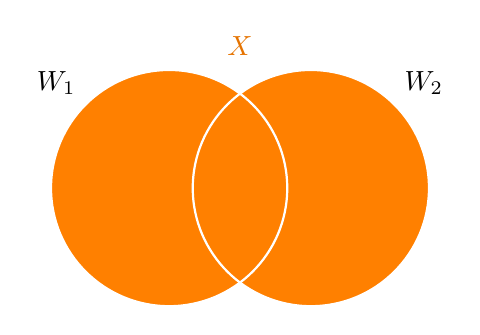
\begin{tikzpicture}
	
	% Set W_1
	\node [circle,
	fill=orange,
	minimum size =3cm,
	label={135:$W_1$}] (W1) at (0,0){};
	
	% Set B
	\node [circle,
	fill=orange,
	minimum size =3cm,
	label={45:$W_2$}] (W2) at (1.8,0){};
	
	% Circles outline
	\draw[white,thick] (0,0) circle(1.5cm);
	\draw[white,thick] (1.8,0) circle(1.5cm);
	
	% Union text label
	\node[orange!90!black] at (0.9,1.8) {$X$};
	
	\end{tikzpicture}
	
	We will show that there exist two closed subsets $A_1$ and $A_2$ of $\tspace$ which satisfy $X_1 \subseteq W_1$ as well as $X_2 \subseteq W_2$ and $X_1 \cup X_2 = X$. Since $\tspace$ satisfies \ref{axiom:t4} and $X \setminus W_2 \subseteq W_1$, there exists an open subset $U$ of $\tspace$ such that $X \setminus W_2 \subseteq U \subseteq \cl{U} \subseteq W_1$. Furthermore, there exists a closed subset $X_2$ of $\tspace$ such that $X \setminus U \subseteq X_2 \subseteq W_2$. This set together with $X_1 := \cl{U}$ are as required, because $X \subseteq \cl{U} \cup \pbraces{X \setminus U} \subseteq X_1 \cup X_2$. 
	
\end{proof}
